% =============================================================
%  - Version: 1.00
% -------------------------------------------------------------
%    Most recent change: 2021.7.21
% =============================================================

%
% =============================================================
%  - Architecture
% -------------------------------------------------------------
\documentclass[AutoFakeBold, AutoFakeSlant, 10pt, aspectratio=169]{beamer}
% =============================================================

% =============================================================
%  - Chinese Support
% -------------------------------------------------------------
\usepackage{xeCJK, fontspec, xunicode, xltxtra}  
% \setmainfont{Courier New} % Pycharm Style
% \setmainfont{CMU Bright} % Beamer Style
% \setCJKmainfont{LXGWWenKaiMono-Regular}
\setCJKmainfont{STKaiti}
\usefonttheme[onlymath]{serif} 
\setlength{\parindent}{2em}

\usepackage{indentfirst}  % 首行缩进
{}\setlength{\parindent}{2em}
% =============================================================

% =============================================================
%  - Utilities
% -------------------------------------------------------------
% Table of Contents
%\setcounter{tocdepth}{3}  % 显示深度
%\setcounter{secnumdepth}{1}  % 编号深度

% Figures
\usepackage{graphicx}

% Tables
\usepackage{longtable}
\usepackage{booktabs}

% Math
\usepackage{amsmath}
\usepackage{amssymb}
\usepackage{extarrows}
\usepackage{mathrsfs}
\usepackage{dsfont}
%\renewcommand\theequation{\thesection.\arabic{equation}}
\numberwithin{equation}{section}  % 方程编号加入章节号
\DeclareMathOperator{\cov}{cov}
\DeclareMathOperator{\var}{Var}

% Frames
\usepackage{framed}
\usepackage[skins,most,theorems]{tcolorbox}

% Parallel Content
\usepackage{paracol}
\usepackage{graphicx,pgf}
\newcommand*{\parallelogramm}{%
  \rlap{\rotatebox{-30}{\rule[.05ex]{.4pt}{.77em}}}%
  \kern.04em%
  \rlap{\kern.36em\raisebox{0.649519052835em}{\rule{.6em}{.4pt}}}%
  \rule{.6em}{.4pt}\kern-.04em%
  \rotatebox{-30}{\rule[.05ex]{.4pt}{.77em}}}

% Hyperlink
% \usepackage{hyperref}
% \hypersetup{pdftex,colorlinks=true,allcolors=blue}
% \usepackage{hypcap}
% \usepackage{hyperref}
% \hypersetup{CJKbookmarks=true, colorlinks=true, citecolor=blue, linkcolor=blue, urlcolor=blue, breaklinks=true}
% =============================================================

% =============================================================
%  - Customize Layout
% -------------------------------------------------------------
% Colors
\usepackage{color}
\definecolor{important}{RGB}{207,54,108}  % 红色
%\definecolor{ans}{RGB}{0,111,255}  % Beamer 主题蓝色
\definecolor{ans}{RGB}{123,150,192}  % 蓝灰色
\definecolor{mark}{RGB}{125,213,195}  % 灰绿色
\definecolor{highlight}{RGB}{253,199,30}  % 橙黄色
\definecolor{qes}{RGB}{140,84,208}  % 紫色

% Spacing between lines
\usepackage{setspace}
\linespread{1.4}
% =============================================================

% =============================================================
%  - My Colorboxes
% -------------------------------------------------------------
% markdown inline codeblock
\definecolor{frame}{RGB}{231,234,237}
\definecolor{back}{RGB}{243,244,244}
\newtcbox{\code}{enhanced,nobeforeafter,tcbox raise base,boxrule=0.4pt,top=0.5mm,bottom=0mm,
  right=0mm,left=0.5mm,arc=1pt,boxsep=2pt,before upper={\vphantom{dlg}},
  colframe=frame,coltext=frame!35!black,colback=back, fontupper=\ttfamily}  % 横向
\MakeRobust\code  % 使可用于标题
% 使 hyperref 可生成标题含该 box 的目录
\ifdefined\pdfstringdefDisableCommands
  \pdfstringdefDisableCommands{\def\mylib#1{'#1'}}
\fi












\begin{document}

\begin{frame}
\title{基于决策树的英雄联盟游戏胜负预测}
\subtitle {实验报告分享}
\author{com.con.} % 显示作者
% \institute {Peking University} % 设置学院机构
\date{Apr 2, 2022}  % 显示日期
\titlepage
\end{frame}

\begin{frame}{任务流程和实验框架}

两条主线:

\begin{itemize}
\item 数据处理: 知道该怎么处理比知道怎么实现数据处理更重要.
\begin{itemize}\setlength{\itemindent}{-1em}
\item[$\circ$] 数据的容器: csv file $\longrightarrow$ pd.DataFrame $\longrightarrow$ np.ndarray $\longrightarrow$ list
\item[$\circ$] 数据的解释: sample $\longrightarrow$ feature $\longrightarrow$ interval $\longrightarrow$ $*$feature\_type
\end{itemize}
\item 算法实现: 根据算法的需求决定数据结构的设计.
\begin{itemize}\setlength{\itemindent}{-1em}
\item[$\circ$] 递归调用: 进度的更新 vs 回溯
\item[$\circ$] 数据结构: 信息的传递 vs 保存
\end{itemize}
\end{itemize}

\end{frame}

\begin{frame}{数据描述与处理}{数据描述}

\vspace{-0.2cm}

要知道怎么处理数据, 首先要了解数据的形式. 以 $*$WardsPlaced 为例:

\begin{figure}[bth]
    \center{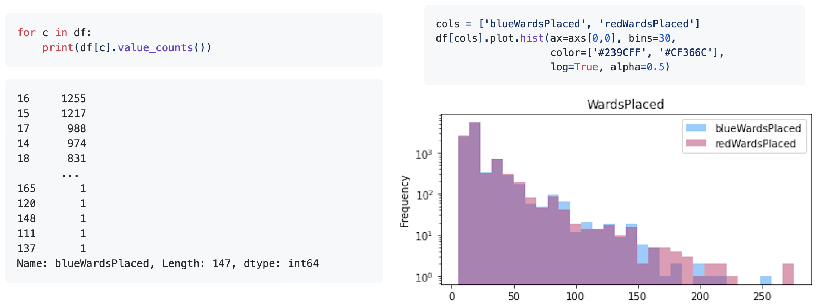
\includegraphics[width=\textwidth]
    {fig/fig1.pdf}}
\end{figure}

\end{frame}

\begin{frame}{数据描述与处理}{数据描述}

\vspace{-0.2cm}

通过上述对取值范围的观察, 可以考虑把特征分成两类:

\vspace{0.2cm}

\begin{figure}[bth]
    \center{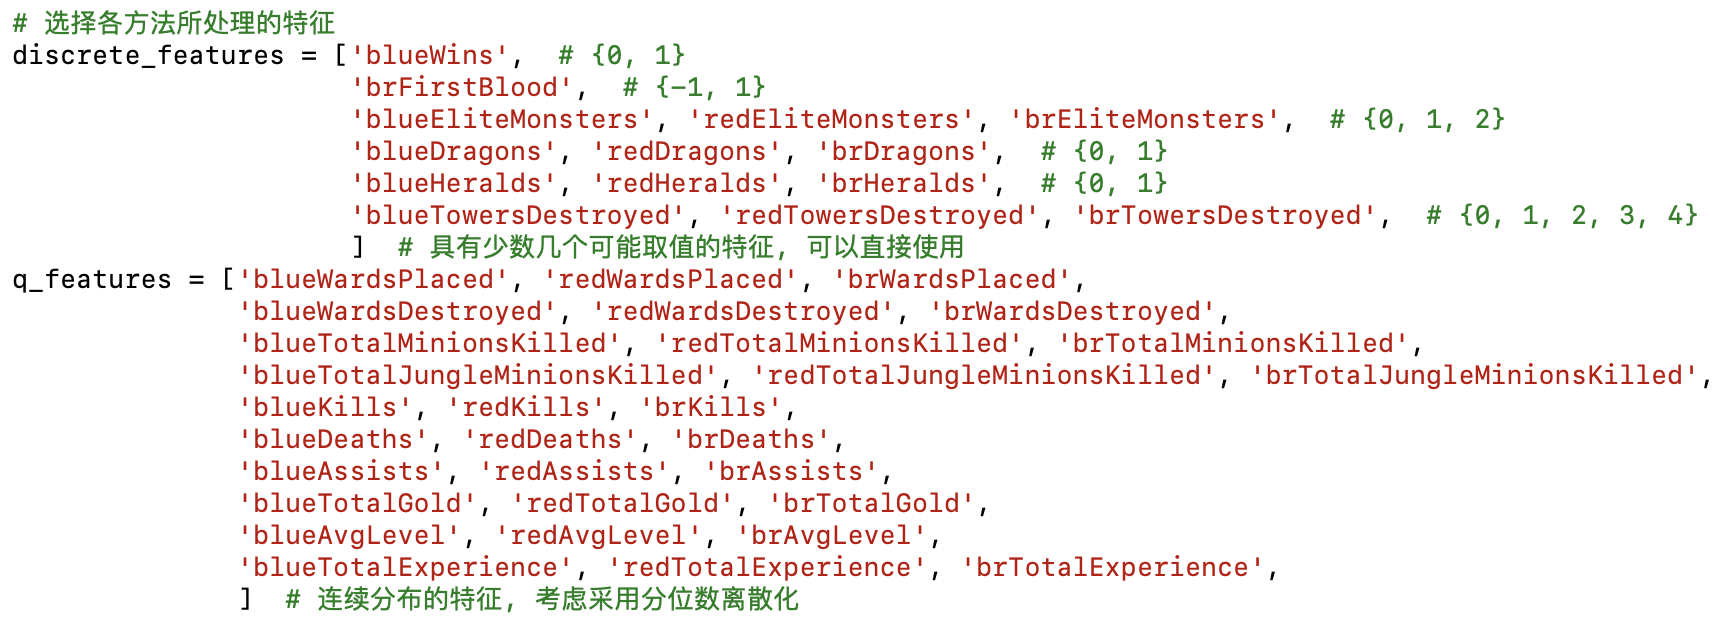
\includegraphics[width=\textwidth]
    {fig/fea_choice.png}}
\end{figure}

\end{frame}

\begin{frame}{数据描述与处理}{数据描述}

\vspace{-0.2cm}

对于取值数目众多的数据类型, 考虑采用分位数对其进行离散化. 这需要观察其分布: 

\vspace{0.3cm}

\begin{figure}[bth]
    \center{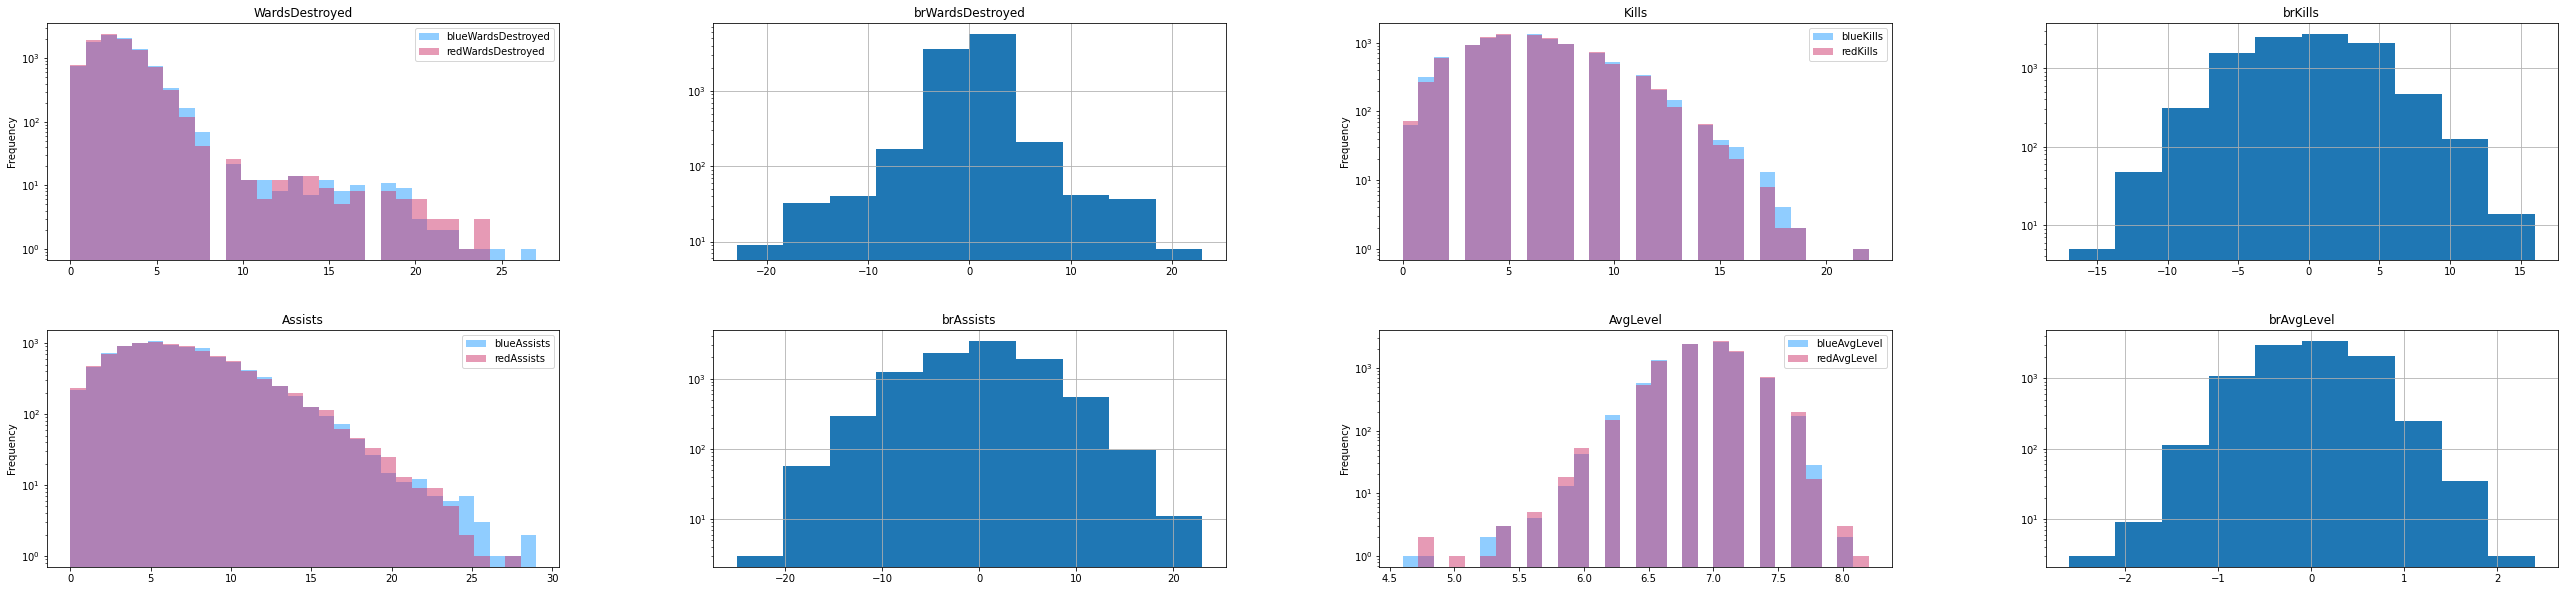
\includegraphics[width=\textwidth]
    {fig/sketch.png}}
\end{figure}

\vspace{0.2cm}
\noindent 观察分布特点, 我们采用以下分位点进行离散化:

\vspace{-0.15cm}
\begin{figure}[bth]
    \center{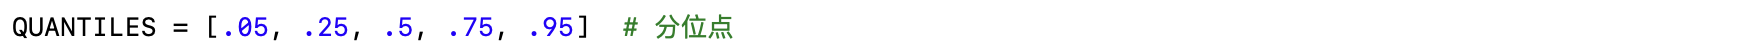
\includegraphics[width=\textwidth]
    {fig/quants.png}}
\end{figure}
\end{frame}

\begin{frame}{数据描述与处理}{数据描述}

\vspace{-0.2cm}

之前的图像中的红蓝色只为了少画两张图, 实际上没有可比性……对数据进一步处理:

\begin{figure}[bth]
    \center{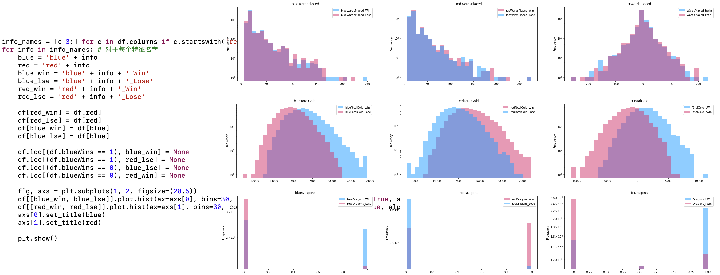
\includegraphics[width=\textwidth]
    {fig/seperaty.pdf}}
\end{figure}

\end{frame}

\begin{frame}{数据描述与处理}{离散化}

\vspace{-0.2cm}

采用以下代码对数据进行离散化:

\vspace{0.1cm}

\begin{figure}[bth]
    \center{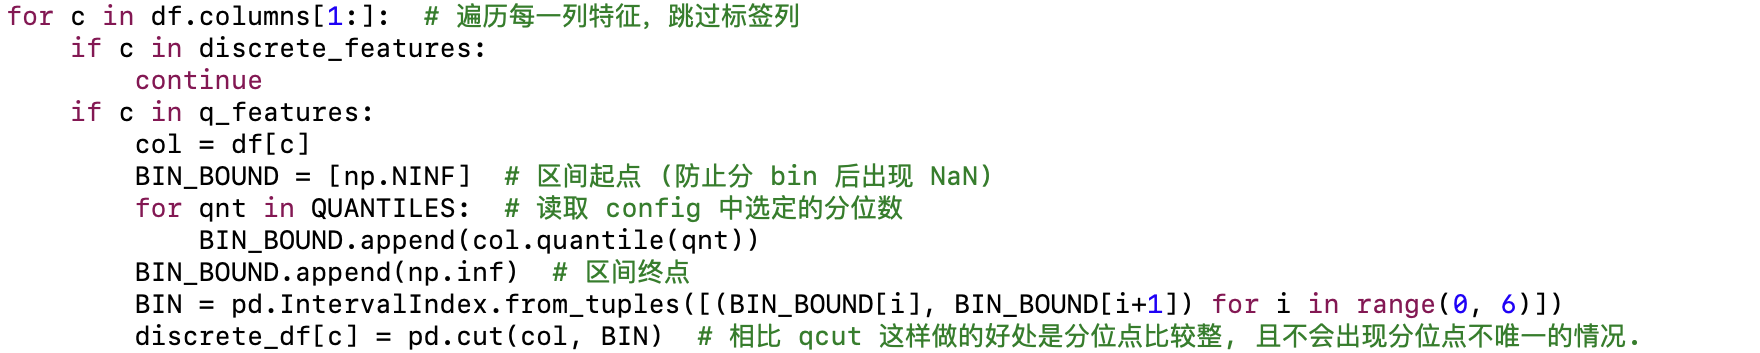
\includegraphics[width=\textwidth]
    {fig/discrete.png}}
\end{figure}

\vspace{0.2cm}

{\linespread{1}\small
\begin{itemize}
\item[注1.] 分位点的起点和终点分别设置为 $-\infty$ 和 $\infty$, 是为了防止划分区间后出现 NaN.
\item[注2.] 分位完成后, 应当检查下分类结果是否正确, 特别地, 检查数据中是否有 NaN.

\vspace{-0.47cm}

\begin{figure}[bth]
    \center{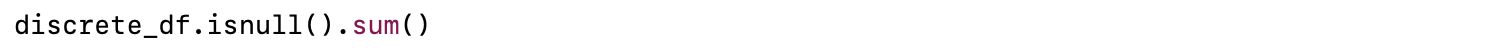
\includegraphics[width=\textwidth]
    {fig/null.png}}
\end{figure}

\vspace{-0.2cm}

\item[注3.] pd.cut vs pd.qcut: 产生 NaN, 可解释性, 唯一性.
\item[注4.] 单独拎出来做判断的方法使得后面舍去部分特征时不需要改参数.
\end{itemize}}
\end{frame}

\begin{frame}{数据描述与处理}{二值化}

\vspace{-0.2cm}

可以进一步对数据做二值化:

\vspace{0.1cm}

\begin{figure}[bth]
    \center{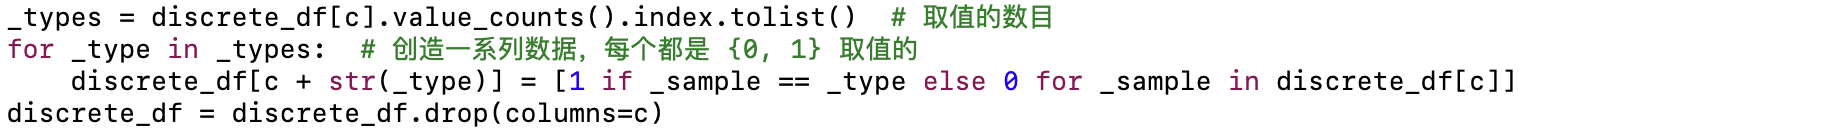
\includegraphics[width=\textwidth]
    {fig/bin.png}}
\end{figure}

\end{frame}

\begin{frame}{算法实现}{输入分析}

\vspace{-0.2cm}

按代码框架形成的训练集, 可以分析每个模型实例需要获知的信息:

\begin{itemize}
\item 数据及其结构, 包括
\begin{itemize}\setlength{\itemindent}{-1em}
\item[$\circ$] 类别的名称 (其实在训练集中也可以获得), 我们约定用一个列表传入
\item[$\circ$] 特征的名称 (训练集中已经 strip 掉了)
\item[$\circ$] 训练集的特征和类别
\end{itemize}

这些东西在生成训练集的代码框架中都已经生成好了, 原样接收即可.

\item 模型的参数, 包括
\begin{itemize}\setlength{\itemindent}{-1em}
\item[$\circ$] 用于预剪枝的参数, 包括最大深度、分裂样本阈值、信息增益阈值等.
\item[$\circ$] 信息熵的计算方法.
\end{itemize}

这些东西的类型也非常直观, 写清楚文档即可.
\end{itemize}

\end{frame}

\begin{frame}{算法实现}{成员设计}

\vspace{-0.2cm}

除了输入信息之外, 为了减少内部函数互相调用时麻烦的传参, 故除上述输入外, 一些不用回溯的数据也被设计成了类的成员. 最终的设计如下:

\begin{figure}[bth]
    \center{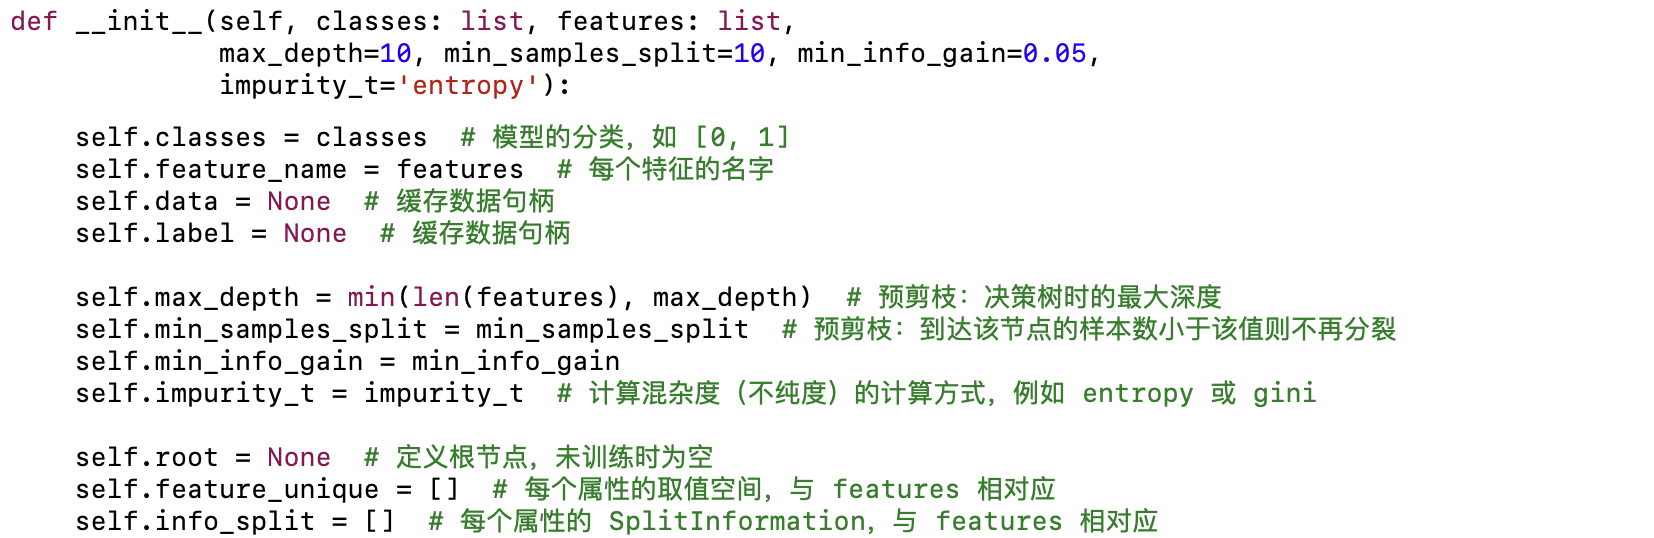
\includegraphics[width=\textwidth]
    {fig/init.png}}
\end{figure}

\end{frame}


% \begin{frame}{算法实现}{熵的计算}

% \vspace{-0.2cm}

% 基于熵运算的结构, 可以抽象出一个统一的接口, 便于传参:

% \begin{figure}[bth]
%     \center{\includegraphics[width=\textwidth]
%     {fig/imp.png}}
% \end{figure}

% \end{frame}

\begin{frame}{算法实现}{模型训练}

\vspace{-0.2cm}

决策树算法基于树, 其核心部分是递归进行. 每次调用中, 需要以下步骤:

\begin{itemize}
\item[(1)] 判断是否到达递归基. 到达递归基后, 需要给当前节点作出分类.
\begin{itemize}\setlength{\itemindent}{-1em}
\item[$\circ$] 无需分裂: 随意取一个样本的类型作为分类即可.
\item[$\circ$] 数目不够或达最大深度: 有样本则少数服从多数; 无样本则跟随父节点类型.  $\longrightarrow$ 需要传参
\item[$\circ$] 没有多余特征: 可以让最大深度不大于特征数解决.
\end{itemize}
\item[(2)] 确定到达当前节点的样本, 以及截至该节点还未被选择的特征. $\longrightarrow$ 需要回溯, 作参数
\item[(3)] 求解该节点上选择每种特征的信息增益, 具体来说, 对每个特征,
\begin{itemize}\setlength{\itemindent}{-1em}
\item[$\circ$] 计算各子节点上的混杂度. $\longrightarrow$ 因为到达每个节点的样本不同, 需要单独统计
\item[$\circ$] 计算惩罚项 Split in Information. $\longrightarrow$ 对每个节点都一样, 可以提前计算
\item[$\circ$] 计算信息增益. $\longrightarrow$ 利用上两步结果, 以及本节点的混杂度 (上一步已计算) 获得, 选择传参
\end{itemize}
\item[(4)] 选出最佳特征, 更新状态, 递归调用.
\end{itemize}

\end{frame}

\begin{frame}{算法实现}{模型训练}

\vspace{-0.2cm}

根据上述分析, 将递归调用部分函数接口设计如下:

\vspace{-0.1cm}

\begin{figure}[bth]
    \center{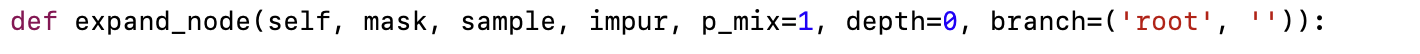
\includegraphics[width=\textwidth]
    {fig/exp.png}}
\end{figure}

\vspace{-0.2cm}

\noindent 其中, 前四个参数分别对应分析中需要传参的可选特征、可选样本、本节点混杂度和父节点的多数特征, 二后两个参数分别用于控制深度和输出信息, 不需参与计算.
\end{frame}

\begin{frame}{算法实现}{模型训练}

\vspace{-1.2cm}

\begin{figure}[bth]
    \center{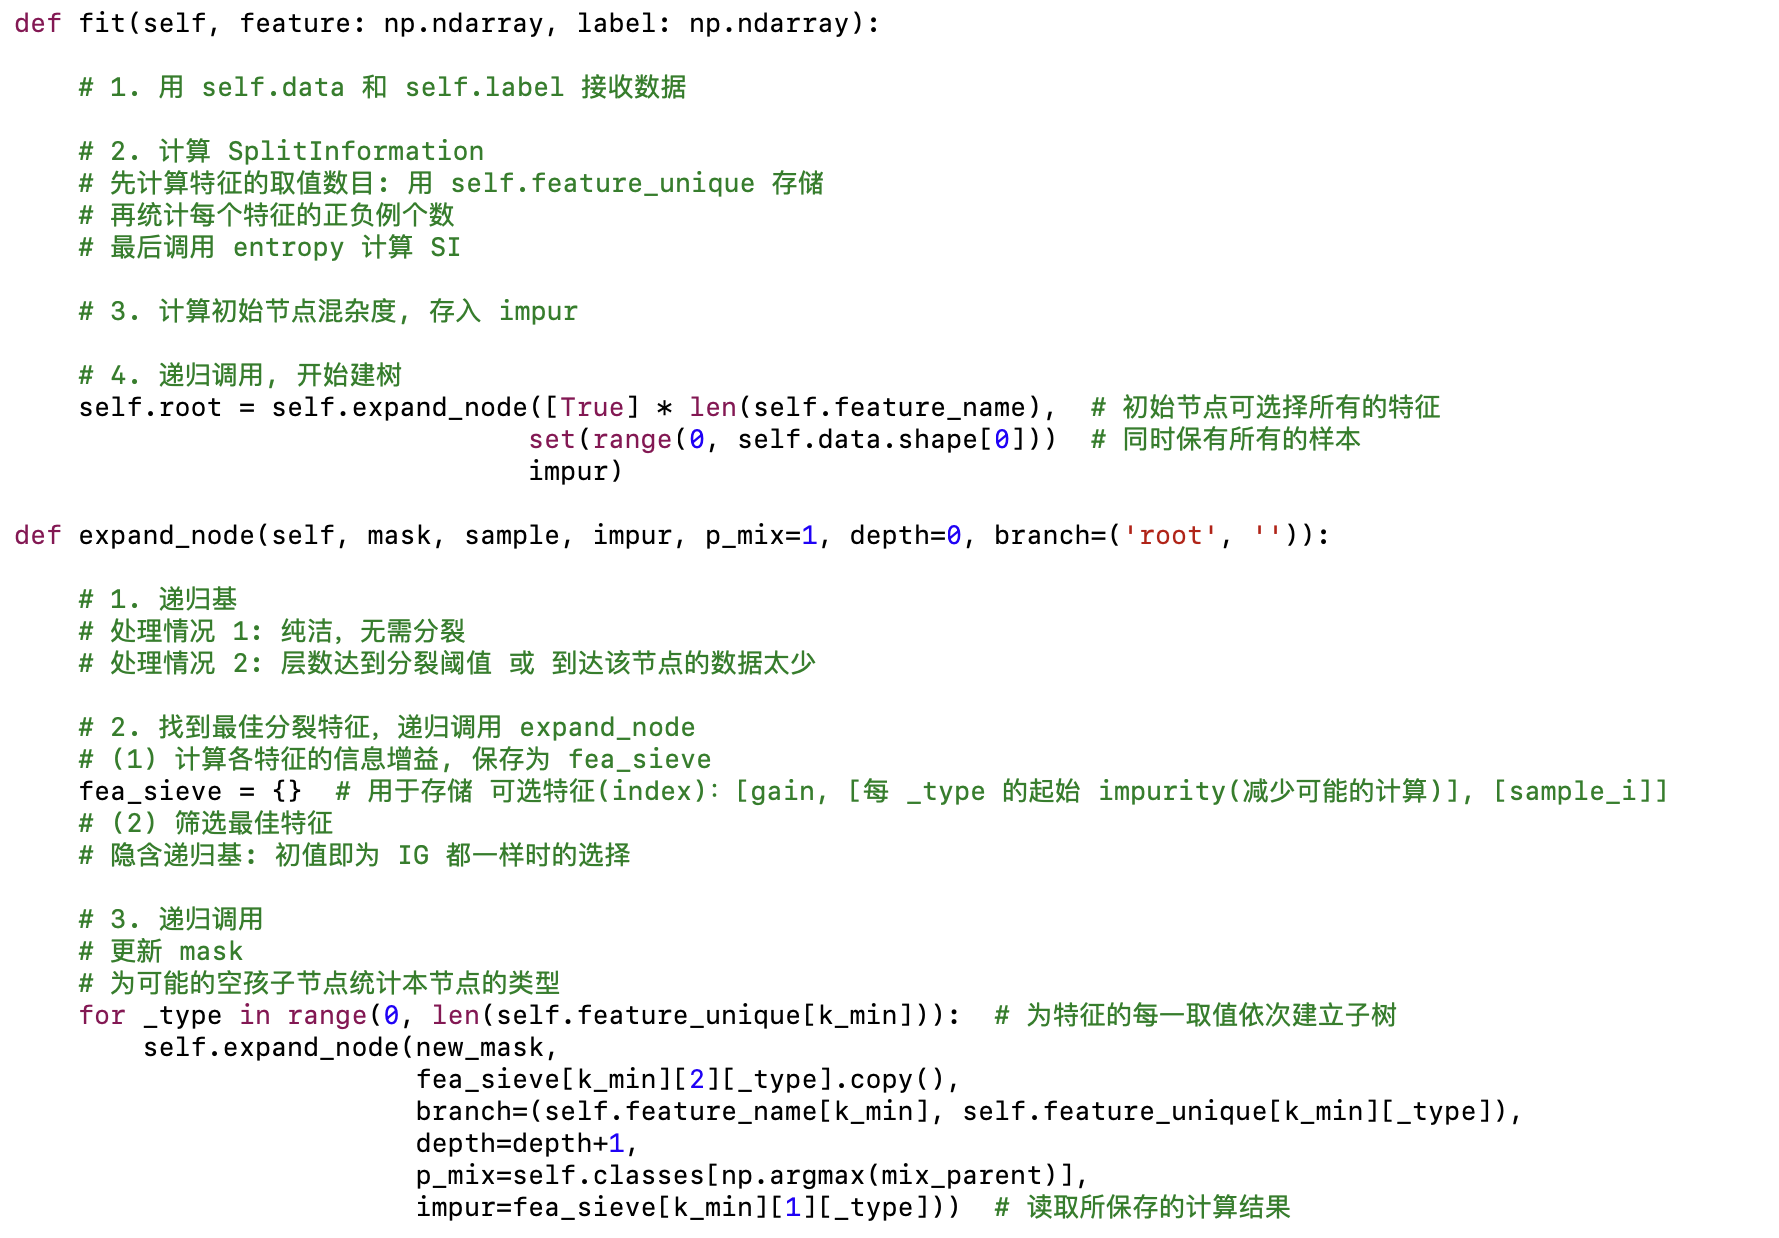
\includegraphics[width=.8\textwidth]
    {fig/outline.png}}
\end{figure}

\end{frame}

\begin{frame}{算法实现}{模型训练}

\vspace{-1cm}

\begin{figure}[bth]
    \center{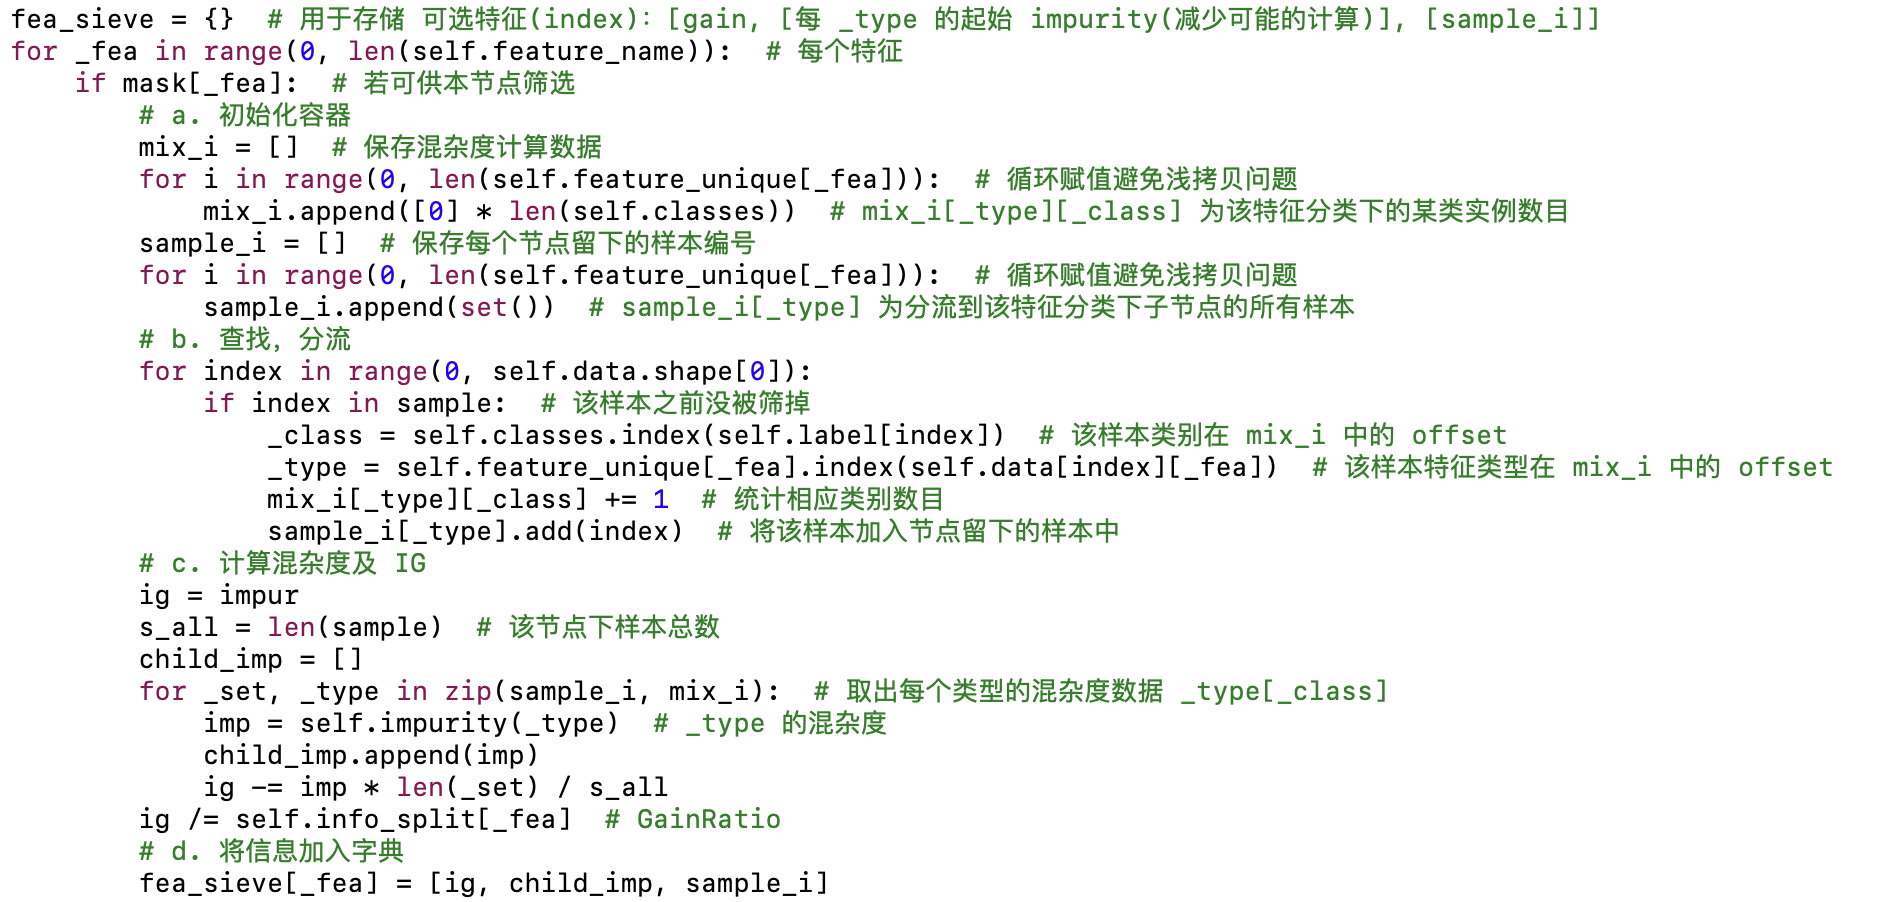
\includegraphics[width=.9\textwidth]
    {fig/count1.png}}
\end{figure}

% \vspace{0.2cm}

{\linespread{1}\small
\begin{itemize}
\item[注1.] 初始化注意浅拷贝问题.
\item[注2.] 对于类别、特征和特征的取值, 都用类成员映射成下标的 offset, 便于应对各种输入.
\end{itemize}}

\end{frame}

\begin{frame}{算法实现}{回溯输出}

\vspace{-0.2cm}

为了保存树的信息和方便回溯输出结果, 定义以下辅助类:

\begin{figure}[bth]
    \center{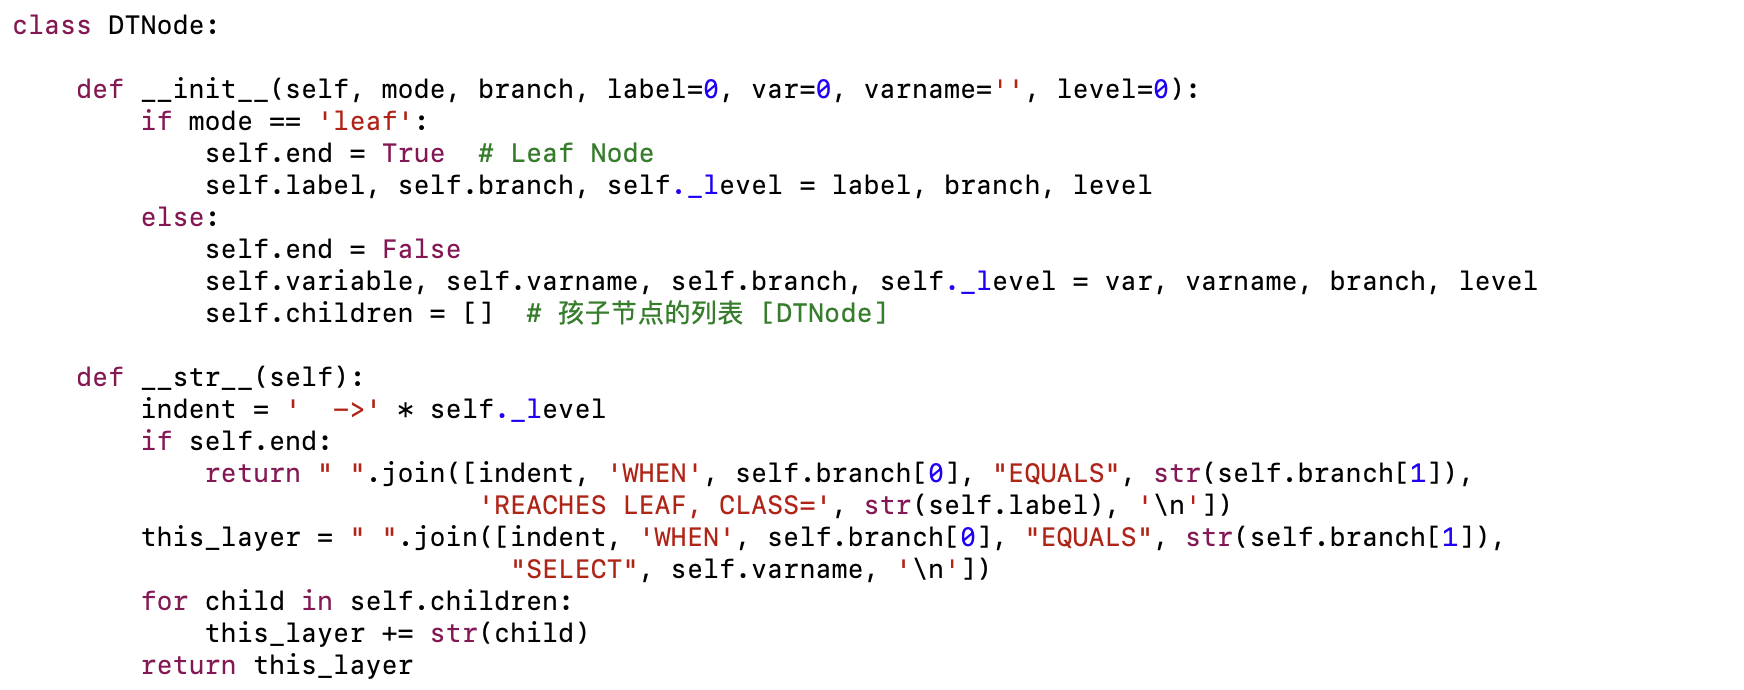
\includegraphics[width=\textwidth]
    {fig/tree.png}}
\end{figure}

\vspace{-0.1cm}

\noindent 这里既要记录辅助输出的信息, 又要记录帮助模型判断的信息.
\end{frame}

\begin{frame}{算法实现}{模型预测}

\vspace{-0.2cm}

模型预测函数在框架中已经给出, 以下是递归调用的实现:

\vspace{-0.1cm}

\begin{figure}[bth]
    \center{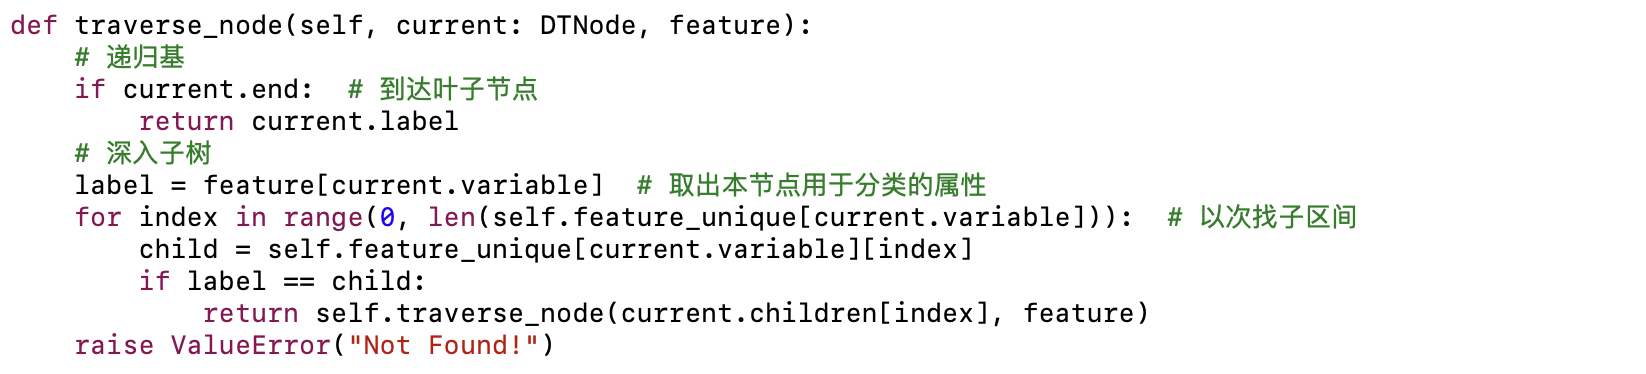
\includegraphics[width=\textwidth]
    {fig/predict.png}}
\end{figure}

\vspace{-0.1cm}

\noindent 事实上如果没有做二值化, 额外加个类型判断还可以对没有离散化的样例进行预测.
\end{frame}

\begin{frame}{模型调优}{参数调整}

\vspace{-0.2cm}

\begin{itemize}
\item 最初的准确率是 0.55. 消除若干处逻辑错误后, 准确率提升到了 0.63.
\item 通过调整最大深度和最小分裂阈值, 准确率提升到了 0.68 (深度 8, 阈值 27). 准确率随二者的变化都是单峰——有一个极大值, 增大或缩小参数都会显著地降低准确率.
\item 调整分位点 QUANTILES:
\begin{itemize}\setlength{\itemindent}{-1em}
\item[$\circ$] 从 QUANTILES 中删除部分分位点数目, 模型准确率大幅下降 (0.59-0.62).
\item[$\circ$] 调整分位点具体位置而不改变分位点数目, 模型准确率略微下降 (0.67-0.68).
\end{itemize}
\item 特征处理方法:
\begin{itemize}\setlength{\itemindent}{-1em}
\item[$\circ$] 只使用特征 blue$* +$ red $*$, 准确率略微提升 (0.68).
\item[$\circ$] 只使用特征 br$*$, 准确率略微下降 (0.67). PS: 一起使用时, 树中也没有选择任何 br$*$.
\item[$\circ$] 对特征进行二值化后, 准确率有小幅提升 (0.70), 但是执行时间显著增加了, 且所需的树的深度增加 (12). 考虑到这样做之后对原始数据进行分类会变得麻烦, 因此是否值得还是一个问题.
\end{itemize}
\item gini 混杂度略优于 entropy (0.67).
\end{itemize}
\end{frame}

\begin{frame}{模型调优}{训练结果}

\vspace{-0.2cm}

\begin{itemize}
\item 可选参数: 深度8, 分裂阈值27, gini 混杂度, 全体特征, 未二值化, 结果准确率为 0.6867.

\vspace{-0.1cm}
\item 最终参数: 深度12, 分裂阈值29, gini 混杂度, 全体特征, 二值化, 结果准确率为 0.7014.
\end{itemize}

\begin{figure}[bth]
    \center{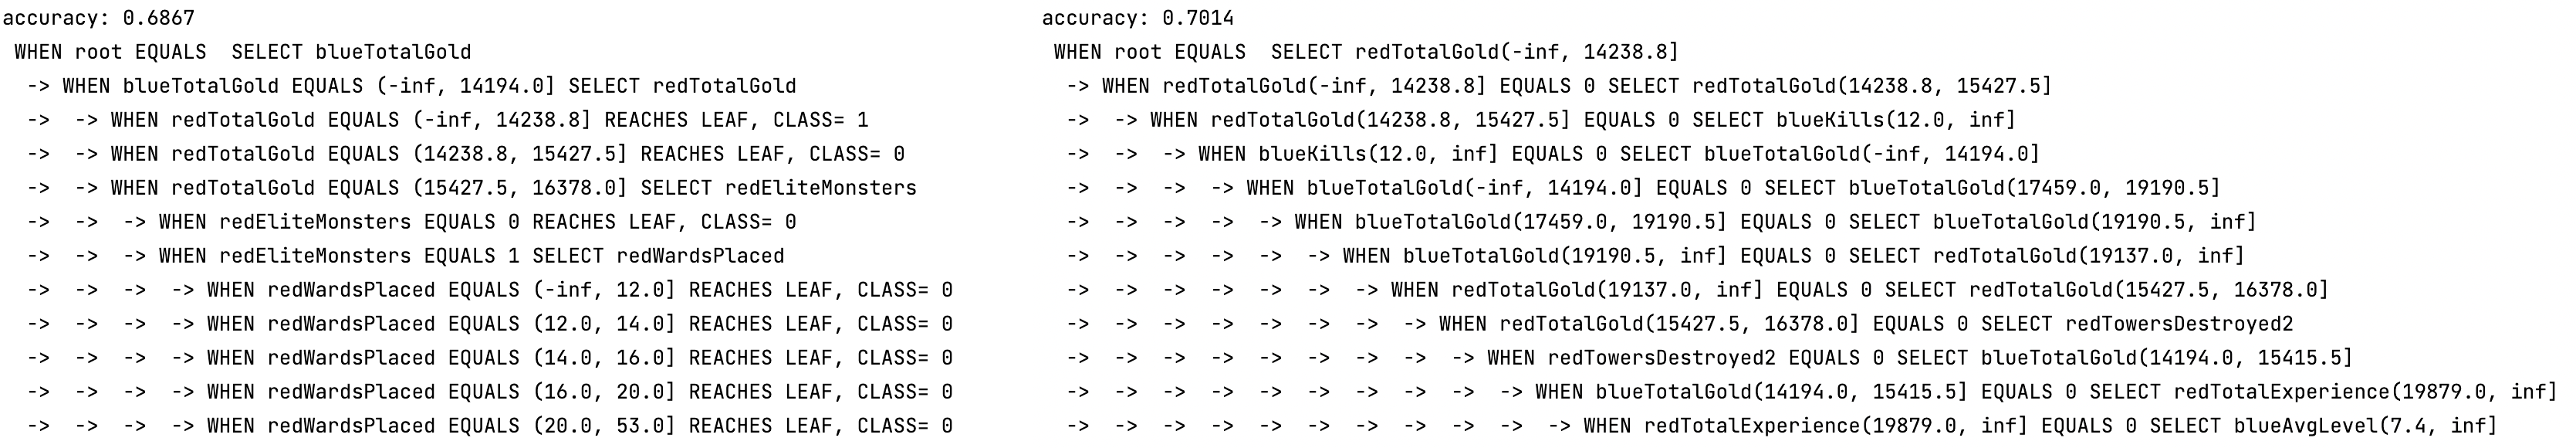
\includegraphics[width=\textwidth]
    {fig/result.png}}
\end{figure}

\begin{itemize}
\item 未来优化方向:
\begin{itemize}\setlength{\itemindent}{-1em}
\item[$\circ$] 实现随机划分 k-fold 验证集.
\item[$\circ$] 使用粒子群算法搜索最优的 QUANTILES 设置 (需要验证集).
\item[$\circ$] 尝试更多特征组合和设置 (需要验证集).
\item[$\circ$] 对决策树实现图形输出.
\end{itemize}
\end{itemize}
\end{frame}







\end{document}